%!TEX root=../GaugeCNNTheory.tex


\subsection{A brief introduction to fiber bundles}
\label{sec:fiber_bundles_general}


Intuitively, a \emph{fiber bundle} can be thought of as a space which is constructed by taking a so called \emph{base space}, in our case the manifold $M$, and attaching another space $F$, denoted as \emph{fiber}, to each of its points.
A trivial example would be the direct product \mbox{$M\times F$}.
However, the fibers can in general be connected in a twisted way such that the resulting bundle is topologically different from a product.
\begin{wrapfigure}[13]{r}{0.54\textwidth}
    \vspace*{-1.4ex}
    \hfill
    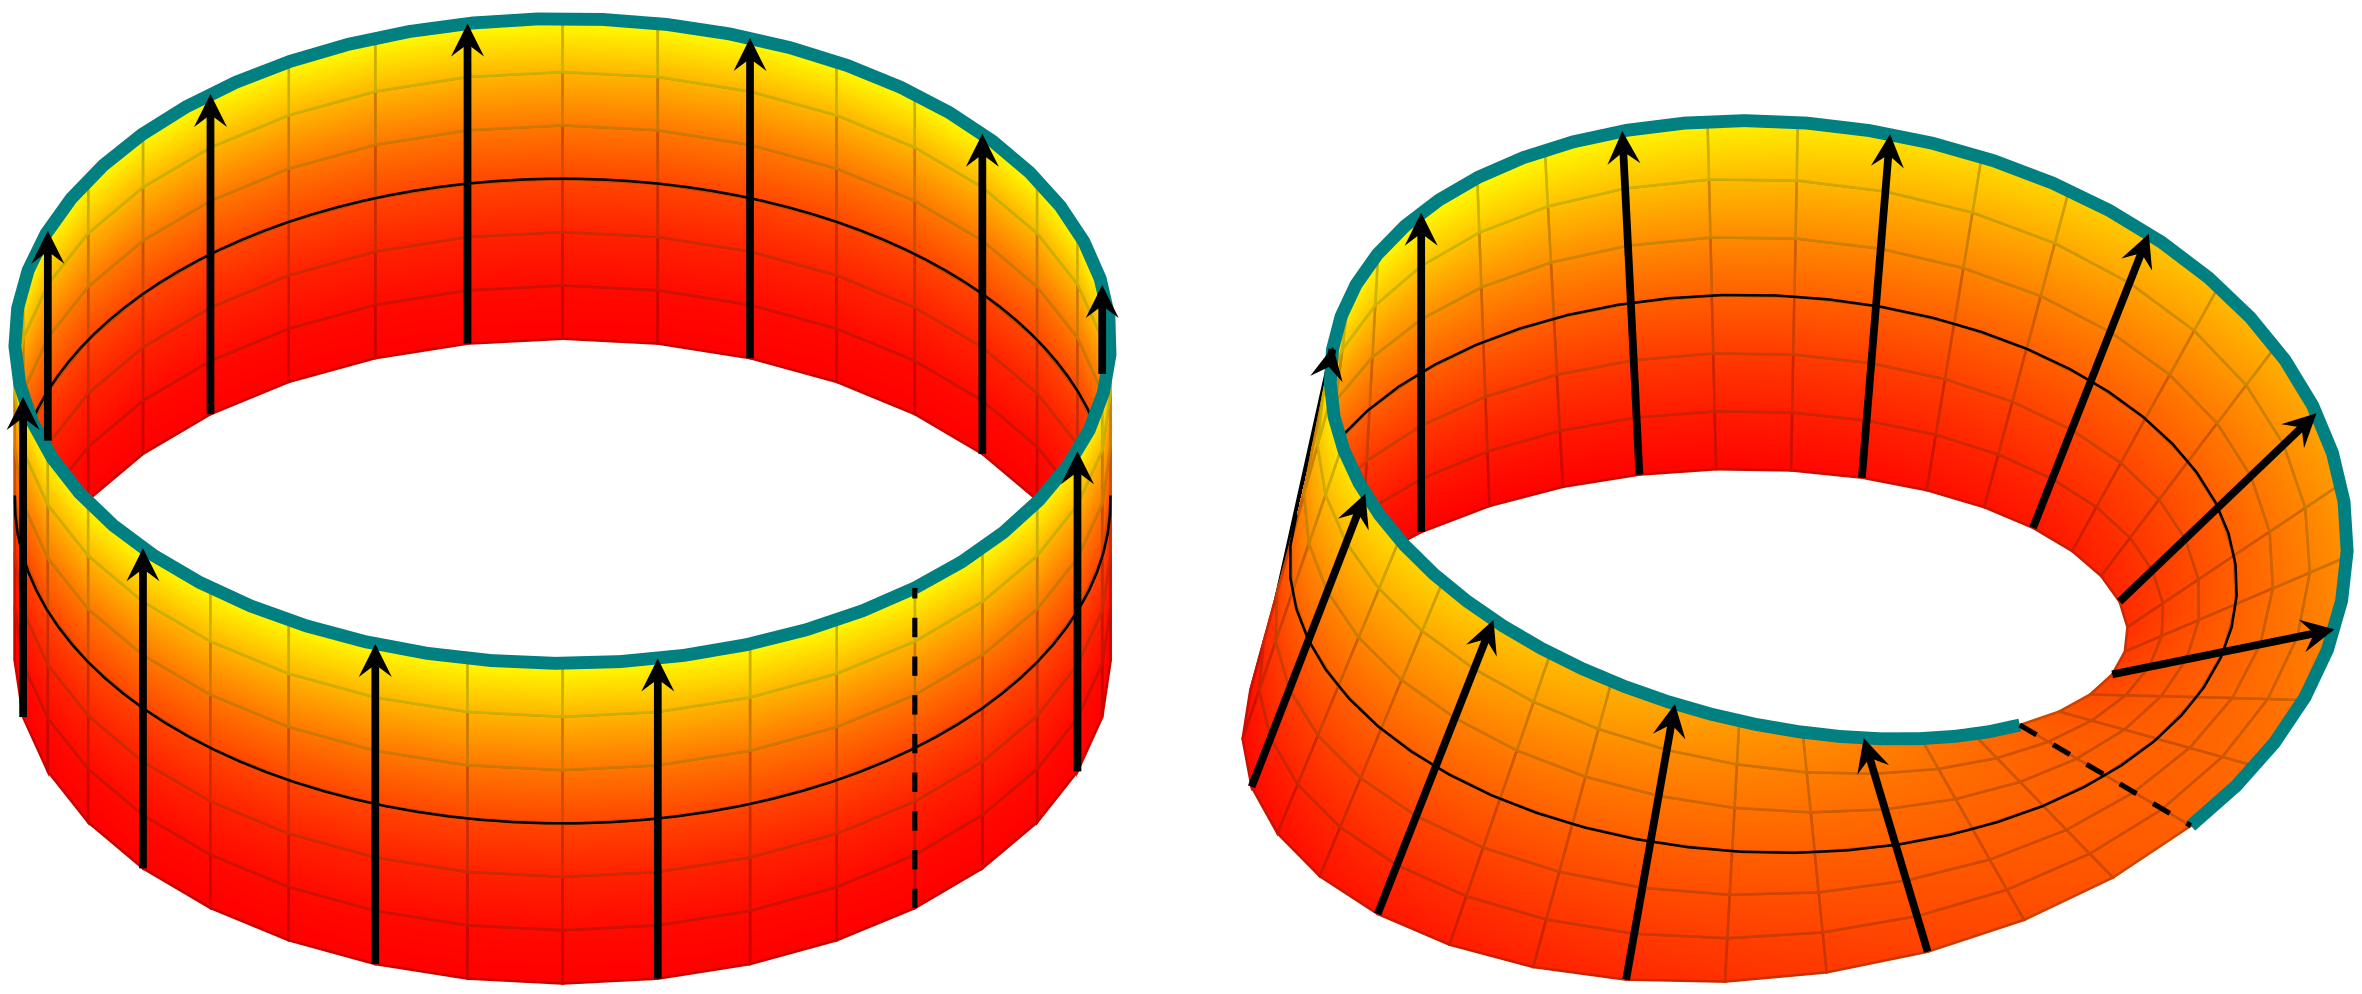
\includegraphics[width=.98\linewidth]{figures/moebius.png}%
    \vspace*{.2ex}
    \caption{\small
        A cylinder and a M{\"o}bius strip.
        Both bundles share the circle $S^1$ as base space and line segments $[-1,1]$ as fibers, however, their topological structure differs by a twist in the fibers.
        {\\
            \color{gray}
            \scriptsize
            (Figure based on Jake's code from
            \href{https://tex.stackexchange.com/questions/118563/moebius-strip-using-tikz}{\underline{tex.stackexchange.com}}.)
        }
        }
    \label{fig:moebius}
\end{wrapfigure}%
For instance, let the base space be the circle $M=S^1$ and let the fiber be the line segment $F=[-1,1]$.
Their direct product $S^1\times[-1,1]$ then forms a cylinder; see Fig.~\ref{fig:moebius} (left).
In contrast, if the fibers are attached such that they are twisted "upside down" after one revolution around the circle, one obtains the M{\"o}bius strip, a non-trivial fiber bundle which is topologically different from the cylinder; see Fig.~\ref{fig:moebius}~(right).%
\footnote{
    To prevent confusion, we emphasize that this example considers the M{\"o}bius strip as a fiber bundle with base space (manifold) $M=S^1$.
    In contrast, all previous figures that contained the M{\"o}bius strip considered it as the base space (manifold) $M$ to convolve over.
}%
\footnote{
    We furthermore need to mention that the arrows shown in the figure are just meant to emphasize the twist in the M{\"o}bius strip.
    They do \emph{not} imply a gluing direction as in \emph{gluing diagrams}.
}
Note that the M{\"o}bius strip \emph{locally} looks like a direct product $U\times F$ of a line element $U\subsetneq S^1$ with the fiber~$F$.
As discussed below, fiber bundles can by definition always be locally trivialized to direct products.


We are interested in fiber bundles since they allow for a global description of fields on manifolds.
For instance, a wind field on the globe $M=S^2$ is a tangent vector field which assigns a tangent vector in $\TpM$ to each point $p$ of~$M$.
The corresponding fiber bundle is the tangent bundle $\TM$ which connects all the tangent spaces together and is therefore identified as a fiber bundle with base space $M=S^2$ and fiber $\R^d\cong \TpM$.
Similar to the fibers of a M{\"o}bius strip, the tangent spaces of a curved manifold are in general not connected in a canonical way but are inherently twisted relative to each other.
The tangent bundle is therefore in general topologically distinct from a product, that is, $\TM \ncong M\times\R^d$.
In order to define $c$-dimensional feature vector fields, we will later consider bundles with base space $M$ and feature vector spaces $\R^c$ as fibers.


\paragraph{Fiber bundles in general:}
Formally, a fiber bundle is a structure $(E,M,\pi,F)$ consisting of topological spaces $E$ (total space), $M$ (base space) and $F$ (typical fiber) and a continuous surjective projection map $\pi:E\to M$.
A fiber bundle is \emph{locally trivializable}, which means that for each point $p\in M$ there exists a local neighborhood $U\subseteq M$ of~$p$, restricted to which the bundle looks like a direct product $U\times F$.
The local triviality is formalized by homeomorphisms%
\footnote{
    A \emph{homeomorphism} is a topological isomorphism, i.e. a continuous, invertible map between topological spaces with continuous inverse.
}
$\Psi:\pi^{-1}(U)\to U\times F$ satisfying the commutative diagram below
\\[-2ex]
\begin{equation}\label{cd:trivialization_general_intro}
\begin{tikzcd}[row sep=3em, column sep=4em]
    \:E\: \supseteq
    &[-4.2em]
    \pi^{-1}(U) \arrow[d, swap, "\pi"] \arrow[r, "\Psi"]
    & U\times F \arrow[ld, "\proj_1"] \\
    M\, \supseteq
    & U
\end{tikzcd}
\quad ,
\end{equation}
that is,
\begin{align}\label{eq:local_triviality_proj}
   \pi\ =\  \proj_1 \circ \mkern2mu \Psi \,,
\end{align}
where $\proj_1: U\times F\to U$ denotes the natural projection on the first factor.
A bundle which is globally homeomorphic to the product $M\times F$ is called \emph{trivial}.
Bundles are often shortly written $E\!\xrightarrow{\pi}\!M$ or just $E$ with the typical fiber and base space left implicit.
Since we are considering smooth frame fields, we assume $E$, $M$ and $F$ to be smooth manifolds and $\pi$ and $\Psi$ to be smooth maps (diffeomorphisms).


The local triviality of $E\!\xrightarrow{\pi}\!M$ implies that the preimage $E_p:=\pi^{-1}(p)$ of any point $p\in M$, called the \emph{fiber over}~$p$, is diffeomorphic to the typical fiber $F$.
As in Section~\ref{sec:gauge_cnns_intro_local}, we denote the diffeomorphisms which identify the fibers over different points with the typical fiber by $\psi_p:E_p\to F$.
The local trivializations are then in terms of these diffeomorphisms given by
\begin{align}\label{eq:Psi_via_psi}
    \Psi:\pi^{-1}(U)\to U\times F,\ \ \ e\mapsto \big(\pi(e),\: \psi_{\pi(e)}(e)\big) \,.
\end{align}
If the typical fiber $F$ and the fibers $E_p$ over $p$ carry additional structure, the diffeomorphisms $\psi_p: E_p\to F$ are required to respect this structure, i.e. to be isomorphisms.%
\footnote{
    Alternatively, assume that $F$ carries structure which is respected by the transition functions $\psi_p^B \circ (\psi_p^A)^{-1} = g^{BA}(p) \in \Aut(F)$ (see the next paragraph).
    Then the trivializations $\psi_p^X: E_p \to F$ consistently \emph{induce} the structure of~$F$ on~$E_p$ and are automatically isomorphisms.
}
For instance, if $F$ and $E_p$ carry a vector space structure, then $\psi_p$ is required to be linear.


In general the specific choice of local trivializations (or diffeomorphisms) over $U$ is not canonically specified by the bundle.
One therefore has to consider different choices (gauges) and \emph{transition functions} (gauge transformations) between them.
To make this precise, consider two overlapping trivializing neighborhoods $U^A$ and $U^B$ with local trivializations $\Psi^A$ and $\Psi^B$.
From Eq.~\eqref{eq:Psi_via_psi} it follows that the transition between both local trivializations is on $U^{AB}:=U^A\cap U^B\neq\varnothing$ given by
\begin{align}\label{eq:transition_function_general_bdl}
    \Psi^B\!\circ\!\big(\Psi^A\big)^{-1}\!:\ U^{AB}\times F \to U^{AB}\times F,
    \quad (p,\mathscr{f}) \mapsto \left(p,\, \pig[\psi_p^B \!\circ\! \big(\psi_p^A\big)^{-1}\, \pig]\mkern-1.5mu(\mathscr{f}) \right)
    =: \left(p,\: g_p^{BA} \,\btr\mkern1.5mu \mathscr{f}\right)
\end{align}
where we implicitly defined the smooth \emph{transition functions}%
\footnote{
    The automorphism group $\operatorname{Aut}(F)$ of a space~$F$ consists of all invertible, structure preserving maps (isomorphisms) from~$F$ to itself.
    For instance, if $F=\R^n$ is a vector space, the automorphism group is the general linear group $\GL{n}$, which consists of all invertible $n\!\times\!n$ matrices.
}
\begin{align}\label{eq:transition_functions_psi}
    g^{BA}: U^{AB} \to \Aut(F),\ \ \ p \mapsto g_p^{BA} := \psi_p^B \circ \big(\psi_p^A\big)^{-1}
\end{align}
and their left action
\begin{align}\label{eq:gauge_trafo_leftaction}
    \blacktriangleright\,:\, \Aut(F) \times F\to F, \quad
    \left(g_p^{BA}, \mathscr{f}\right) \;\mapsto\; g_p^{BA}\,\btr\mkern1.5mu \mathscr{f} \;:=\; \left[\psi_p^B\circ\big(\psi_p^A\big)^{-1}\right]\!(\mathscr{f}).
\end{align}
on the typical fiber $F$; cf. Eqs.~\eqref{eq:gauge_trafo_local_def_21} and~\eqref{eq:transition_fct_local_def_21}.
To see that the first factor in Eq.~\eqref{eq:transition_function_general_bdl} is indeed given by the identity, note that, for any $p\in U^{AB}$ and any $\mathscr{f}\in F$, the repeated application of Eq.~\eqref{eq:local_triviality_proj} implies
$
    \pig[ \proj_1 \circ \Psi^B \circ \big(\Psi^A\big)^{-1} \mkern1mu\pig] (p,\mathscr{f})
    \ =\ \pig[ \pi \circ \big(\Psi^A\big)^{-1}  \mkern1mu\pig] (p,\mathscr{f})
    \ =\ \proj_1 (p,\mathscr{f})
    \ =\ p \,.
$
The transition between different trivializations is visualized by the following (commuting) extension of the commutative diagram in Eq.~\eqref{cd:trivialization_general_intro}:
\begin{equation}\label{cd:trivialization_general_trafo}
\begin{tikzcd}[row sep=3.5em, column sep=5.em]
    U^{AB}\!\times\!F
        \arrow[rd, "\proj_1"']
        \arrow[rr, rounded corners, to path={ 
                    -- ([yshift=4ex]\tikztostart.north) 
                    --node[above, pos=.5]{\small$\id \times g^{BA}\btr$} ([yshift=4ex]\tikztotarget.north) 
                    -- (\tikztotarget.north)
                    }]
    & \pi^{-1}(U^{AB})
        \arrow[d, swap, "\pi"]
        \arrow[l, "\Psi^A"']
        \arrow[r, "\Psi^B"]
    & U^{AB}\!\times\!F
        \arrow[ld, "\proj_1"]
    \\
    & U^{AB}
\end{tikzcd}
\end{equation}
Restricted to a single point $p\in U^{AB}$, and for the specific case of the tangent bundle (defined below), this diagram corresponds to that in Eq.~\eqref{eq:commutative_diagram_TpM} and its graphical version in Fig~\ref{fig:gauge_trafos}.


By definition, the transition functions in Eq.~\eqref{eq:transition_functions_psi} satisfy the following three conditions:%
\footnote{%
    Conditions $i)$ and $ii)$ follow from the cocycle condition $iii)$ but are often stated explicitly.
}
\begin{alignat}{3}
       i) \qquad&& g_p^{AA}         \;&=\ e                     \quad&&\forall p\in U^A \label{eq:transition_condition_1}\\
      ii) \qquad&& g_p^{BA}         \;&=\big(g_p^{AB}\big)^{-1} \quad&&\forall p\in U^A\cap U^B \label{eq:transition_condition_2}\\
     iii) \qquad&& g_p^{CB} g_p^{BA}\;&=\ g_p^{CA}              \quad&&\forall p\in U^A\cap U^B\cap U^C \qquad \text{(cocycle condition)} \label{eq:transition_condition_3}
\end{alignat}
By the \emph{fiber bundle construction theorem}, any fiber bundle can be fully specified globally in terms of an \emph{atlas}
$\mathscr{A}\ =\ \big\{\big( U^X, \Psi^X \big) \,\big|\, X\in\mathfrak{X} \big\}$
of local trivializations $\big(U^X,\Psi^X\big)$ which cover $M$ and whose transition functions satisfy Eqs.~\eqref{eq:transition_condition_1}, \eqref{eq:transition_condition_2} and~\eqref{eq:transition_condition_3} (here $\mathfrak{X}$ denotes some index set).
The individual trivializations can be thought of as being ``glued together'' by the transition maps, which is visualized in Fig.~\ref{fig:trivializations_moebius}.
Note that this is similar to the global description of a manifold in terms of an atlas of local charts.










\paragraph{Vector bundles:}
Several more specific notions of fiber bundles, carrying additional mathematical structure, exist.
An important example are \emph{vector bundles}, which, as the name suggests, are bundles consisting of vector spaces attached to a manifold.
Formally, a (real) vector bundle of rank~$k$ is a bundle $(E,M,\pi,\R^k)$ with typical fiber~$\R^k$ and fibers $E_p \cong \R^k$ over $p$ such that the local trivializations are fiber wise vector space isomorphisms (linear maps).
The transition functions $\psi^B_p \circ \big(\psi^A_p\big)^{-1} \in \Aut(\R^k) = \GL{k}$ then take values in the general linear group.

Alternatively, given the fiber $\R^k$ and an atlas of local trivializations whose transition functions take values in $\Aut(\R^k) = \GL{k}$, a vector space structure of $E_p$ is induced by setting
\begin{align}
    \alpha v + \beta w \ :=\ \big(\psi_p^A \big)^{-1} \big( \alpha \psi_p^A(v) + \beta \psi_p^A(w) \big) \qquad \forall\ v,w\in E_p,\ \ \alpha,\beta\in\R
\end{align}
for an arbitrary gauge $\psi_p^A: E_p \to \R^k$ from the $\GL{k}$-atlas.
That the vector space structure is consistently defined is clear as
\begin{align}
       &\big( \psi_p^B \big)^{-1} \pig( \alpha \psi_p^B(v) + \beta \psi_p^B(w) \pig) \notag \\
    =\ &\big( \psi_p^A \big)^{-1} \pig( \big(g^{BA}_p)^{-1} \big( \alpha g^{BA}_p \psi_p^A(v) + \beta g^{BA}_p \psi_p^A(w) \big) \pig) \notag \\
    =\ &\big( \psi_p^A \big)^{-1} \pig( \alpha \psi_p^A(v) + \beta \psi_p^A(w) \pig)
\end{align}
yields the same result.
Note that the last step required the linearity of $g_p^{BA} \in \GL{d}$.
The gauges $\psi_p^A$ or $\psi_p^B$ are then automatically vector space isomorphisms.

The most relevant examples for us are the tangent bundle and feature vector bundles, which are introduced in the following sections.










\paragraph{\textit{G}-bundles}
Depending on the topology of the bundle, it might be possible to define an atlas of local trivializations
$\mathscr{A}^G\ =\ \big\{\big( U^X, \Psi^X \big) \,\big|\, X\in\mathfrak{X} \big\}$
whose \emph{transition functions are restricted to a subgroup} ${G \leq \Aut(F)}$, that is, they satisfy
\begin{align}
    g_p^{BA} \in G\quad\ \ \textup{for all}\ \ A,B\in\mathfrak{X}\ \ \textup{and all}\ \ p\in U^A\cap U^B \,.
\end{align}
Any such atlas is called $G$-\emph{atlas} and $G$ is denoted as \emph{structure group} of the bundle.
Two different $G$-atlases are equivalent (or compatible), if their union is again a $G$-atlas.
A bundle equipped with an equivalence class of $G$-atlases is known as a $G$-bundle.%
\footnote{
    The equivalence class ensures thereby that no single of the equivalent $G$-atlases is preferred.
    Equivalently, one could take the \emph{maximal} $G$-atlas, defined as the unique $G$-atlas in which any other compatible $G$-atlas is contained.
    Note that an equivalence class of $G$-atlases is uniquely implied by a single given $G$-atlas.
}

\begin{figure*}
    \centering
    \begin{subfigure}[b]{0.46\textwidth}
        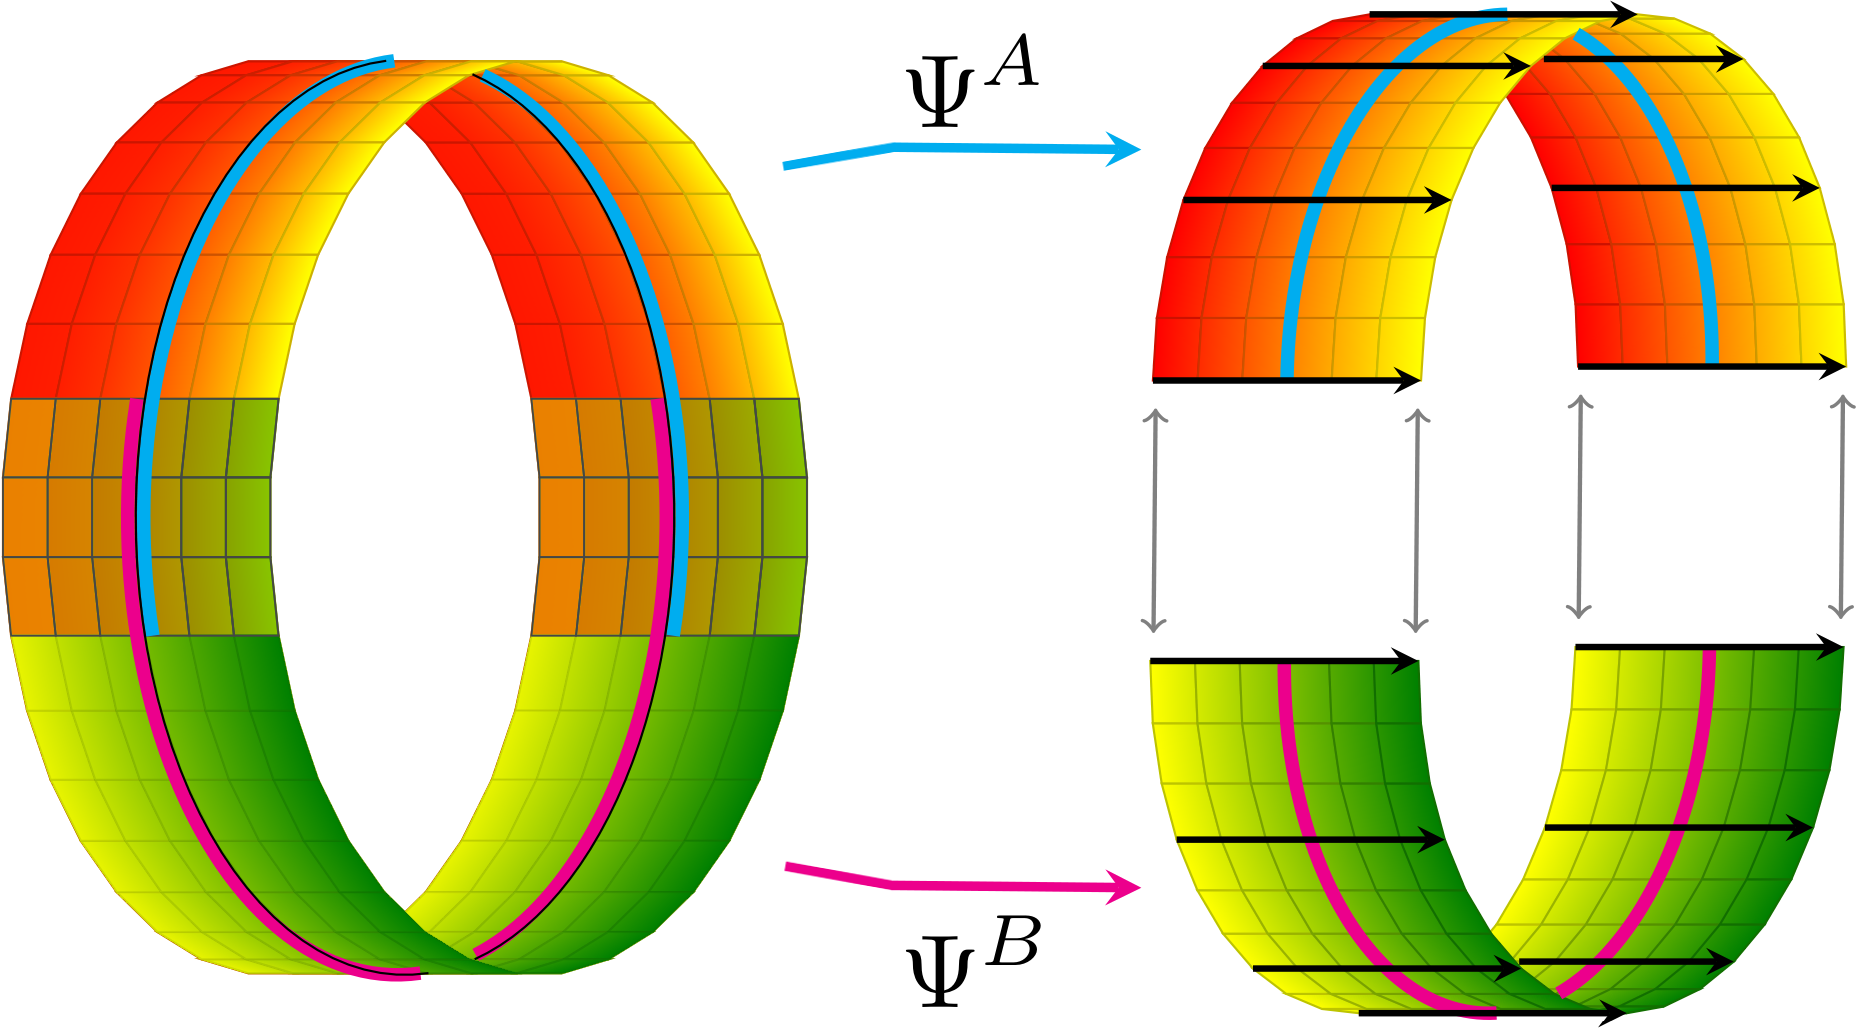
\includegraphics[width=\textwidth]{figures/trivialization_cylinder.png}
    \end{subfigure}
    \hfill
    \begin{subfigure}[b]{0.46\textwidth}
        \centering
        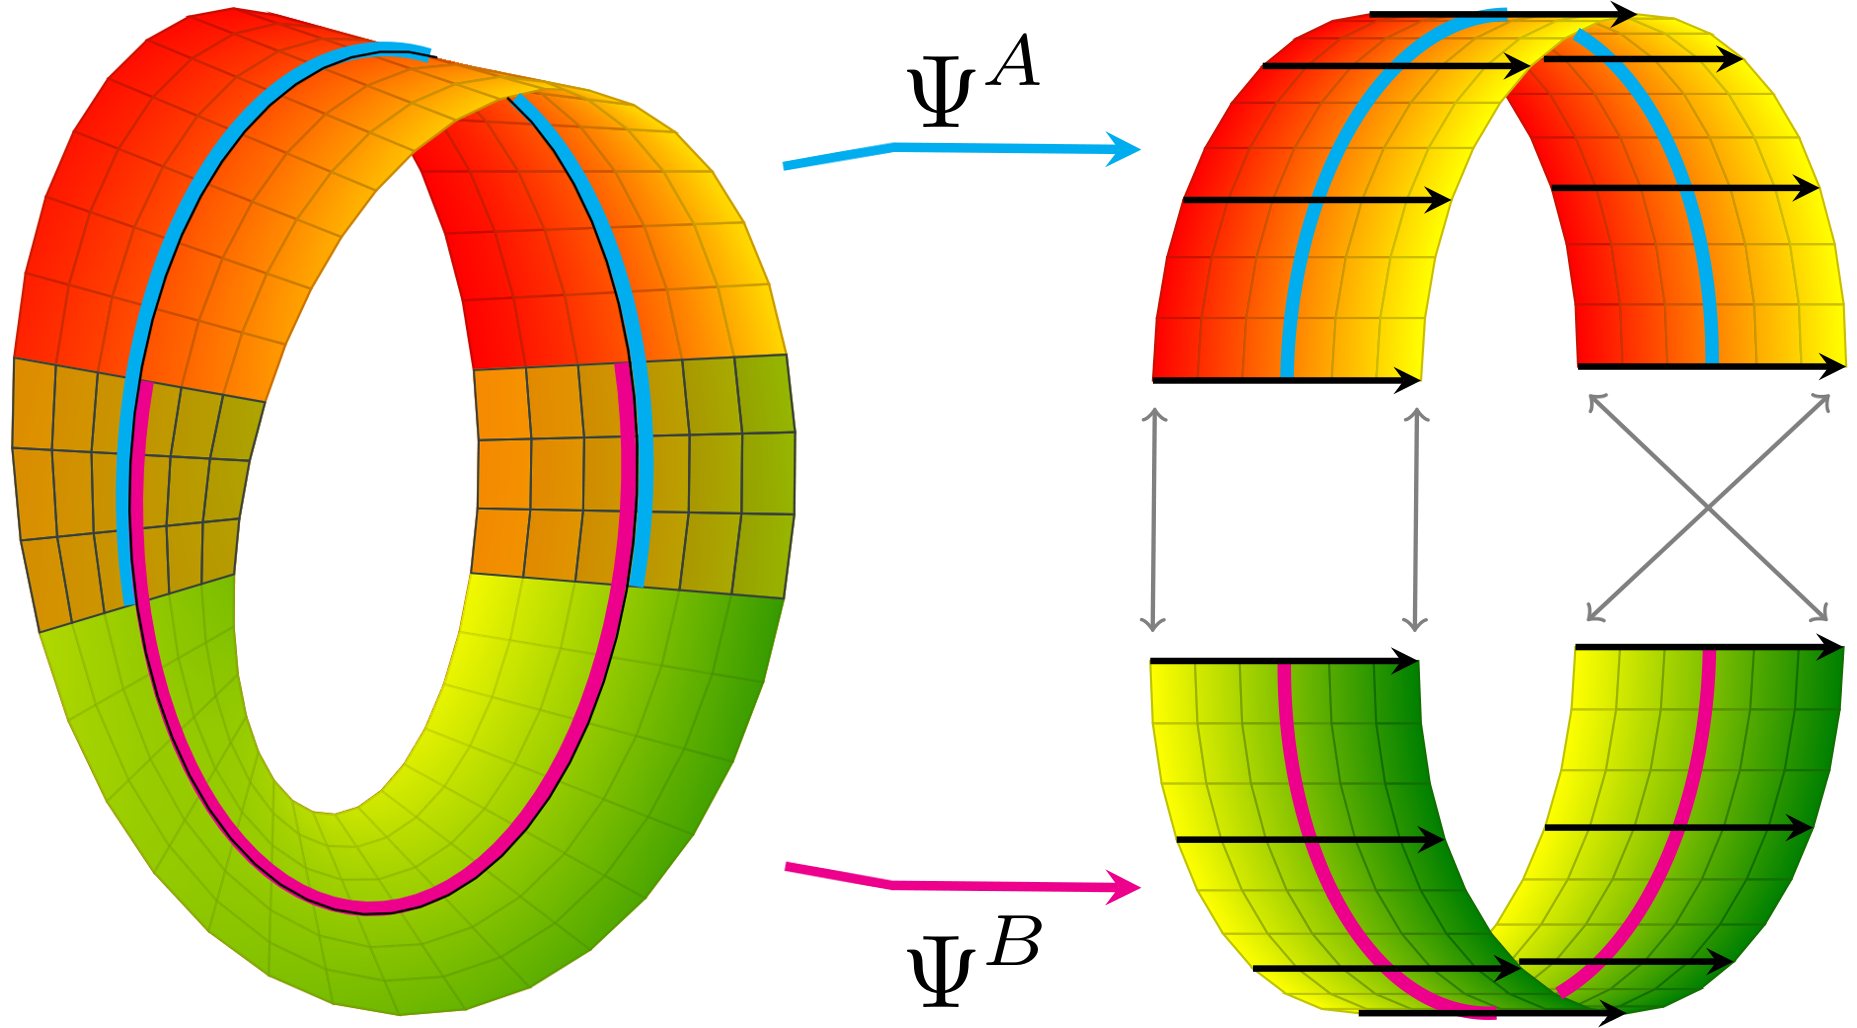
\includegraphics[width=\textwidth]{figures/trivialization_moebius_2.png}
    \end{subfigure}
    \vspace{2.ex}
    \caption{\small
        Description of the cylinder and the M{\"o}bius strip in terms of $G$-atlases consisting of two local trivializations each.
        \textit{Left:}~Since the cylinder is a trivial bundle, all transition functions can be chosen to be identity maps such that the structure group is reduced to the trivial group $G=\{e\}$.
        Differing from the visualized situation, it is possible to choose a single, global trivialization.
        \textit{Right:}~The topology of the M{\"o}bius strip forces the transition functions at one of the overlaps to glue the fibers together in an inverted way.
        The structure group can therefore not be reduced further than the group $G=\Flip$ which models the reflection of fibers.
        Global trivializations of the M{\"o}bius strip do therefore not exists.
        Note that the arrows on the M{\"o}bius strip should not be confused with the arrows in gluing diagrams, that is, the twist glues the vectors at one of the cuts in opposite direction.
    }
    \label{fig:trivializations_moebius}
\end{figure*}

The topology of a bundle determines how far its structure group can be reduced.
For instance, the cylinder in Fig.~\ref{fig:trivializations_moebius} (or any other trivial bundle) can be described by an $\{e\}$-atlas, consisting of local trivializations with identity transition functions only.
This corresponds to a reduction to a trivial structure group $G=\{e\}$.
In contrast, the twisted topology of the M{\"o}bius strip requires any $G$-atlas to contain transition functions which glue the fibers together in an inverted orientation; see Fig~\ref{fig:trivializations_moebius} (right).
The structure group of the M{\"o}bius strip can therefore not be restricted further than the group $G=\Flip$ which models the reflection of fibers.
On Riemannian manifolds the structure group of the tangent bundle $\TM$, and thus the associated feature vector bundles, can in general not be reduced further than to an orthogonal structure group $\O{d}$ which motivated this work on coordinate independent CNNs in the first place.








\paragraph{Associated \textit{G}-bundles:}
Two $G$-bundles are said to be \emph{associated} to each other if they share the same base space, structure group and, most importantly, \emph{same transition functions}.
Associated bundles $(E,M,\pi,F)$ and $(\widetilde{E},M,\widetilde{\pi},\widetilde{F})$ with structure group $G$ might differ in their typical fibers~$F$ and $\widetilde{F}$ and therefore also in their left actions $\blacktriangleright: G \times F\to F$ and $\widetilde{\blacktriangleright}: G \times \widetilde{F}\to \widetilde{F}$ of~$G$ on the respective fiber.
Given two $G$-atlases
$\big\{\big( U^X,            \Psi^X  \big) \,\big|\, X\in\mathfrak{X} \big\}$ and
$\big\{\big( U^X, \widetilde{\Psi}^X \big) \,\big|\, X\in\mathfrak{X} \big\}$
of the bundles over the same open cover of $M$, the requirement for the equivalence of the transition functions (up to the different left actions) means:
\begin{align}
    \Psi^B \circ \big(\Psi^A \big)^{-1}\ =\ \big(\id \times g^{BA}\blacktriangleright \big)
    \qquad \Longleftrightarrow \qquad
    \widetilde{\Psi}^B \circ \big(\widetilde{\Psi}^A \big)^{-1}\ =\ \big(\id \times g^{BA}\, \widetilde{\blacktriangleright} \big)
\end{align}
Intuitively, the typical fibers~$F$ and~$\widetilde{F}$ of~$E$ and~$\widetilde{E}$ are ``glued together'' in the same way over~$M$.

An important example of bundles which are $\GL{d}$-associated to each other are the tangent bundle $\TM$, the cotangent bundle $\TsM$, any other tensor bundle $\TrsM$ and the tangent frame bundle~$\FM$, (the first and the latter are introduced in Section~\ref{sec:GL_associated_bundles}).
The associatedness of these bundles is reflected in that their components relative to chosen bases transform according to the same gauge transformation (e.g. Jacobian $g^{BA}_{\mu\nu} = \frac{\partial x^B_\mu}{\partial x^A_\nu}$, see Appendix~\ref{apx:coordinate_bases}).
The different actions of a gauge transformation on the respective fibers is in this example denoted as being a contravariant transformation ($\TM$), covariant transformation ($\TsM$), $r$-times contra- and $s$-times covariant transformation ($\TrsM$) and, again, covariant transformation ($\FM$), respectively.
We will later on introduce the $G$-structure $\GM$, the tangent bundle $\TM$ and the feature vector bundles $\A$ as associated $G$-bundles.
The associatedness does in this case come from the fact that changes of reference frames in $\GM$ lead to a simultaneous transformations of the tangent vector coefficients and feature vector coefficients.

We want to mention that any associated bundles are additionally associated to a uniquely specified principal $G$-bundle (defined in the next paragraph).
In turn, any associated bundle can be constructed from the respective associated principle bundle -- we will make heavy use of this construction to define feature vector bundles in Section~\ref{sec:G_associated_bundles}.








\paragraph{Principal \textit{G}-bundles:}
A fiber bundle $(P,M,\pi,G)$ is called a (smooth) \emph{principal G-bundle} $(P,M,\pi,G,\lhd)$ if 1) its typical fiber coincides with its structure group $G$ and 2) it is endowed with a smooth \emph{right $G$-action}
\begin{align}
    \lhd: P \times G \to G,\ \ (\mathscr{p},g) \mapsto \mathscr{p}\lhd g
\end{align}
which preserves the fibers, that is,
\begin{align}
    \pi(\mathscr{p}\lhd g)\ =\ \pi(\mathscr{p})\quad \forall\ \mathscr{p}\in P,\ g\in G
\end{align}
and acts \emph{transitively} and \emph{freely} on them.%
\footnote{%
    A (right) group action $\phi:X\times G\to X,\ (x,g)\mapsto x.g$ is called \emph{transitive} if any point of $X$ can be mapped to any other point i.e. if for each $x,y\in X$ there exists a $g\in G$ such that $y=x.g$.
    It is called (fixed point) \emph{free} if for any $x\in X$ the equation $x=x.g$ implies that $g=e$, that is, if only the action of the identity element leaves $p$ invariant.
    Note that the same statements can be made for left actions.
}
The last two conditions (transitivity and freedom) together require that the fibers of a principal $G$-bundle are $G$-torsors (or principal homogeneous $G$-spaces), which intuitively means that they ``look like~$G$'' but come without any specified origin or identity element.%
\footnote{
    Formally, a (right) $G$-torsor $P$ satisfies $P\times G \cong P\times P$ where the isomorphism is given by $(p,g) \mapsto (p,p.g)$.
    This condition implies that there is a \emph{unique} group element connecting \emph{any} two points in the torsor.
}
The local trivializations $\Psi: \pi^{-1}(U) \to U \times G$ are required to respect the right $G$-action, that is, to be right $G$-equivariant
\begin{align}\label{eq:right_G_equiv_principal_bdl_general}
    \Psi(\mathscr{p} \lhd g)\ =\ \Psi(\mathscr{p}) (\id \times \cdot\mkern1mu g)
    \quad \textup{or, equivalently,}\quad
    \psi_{\pi(\mathscr{p})} (\mathscr{p}\lhd g)\ =\ \psi_{\pi(\mathscr{p})} (\mathscr{p}) \cdot\mkern0mu g
    \qquad \forall\ \mathscr{p}\in P,\ g\in G \,,
\end{align}
where $\cdot g$ denotes the canonical right multiplication with group elements on the typical fiber~$G$.
This extends the diagram in Eq.~\eqref{cd:trivialization_general_intro} to the diagram
\begin{equation}\label{cd:trivialization_principal_intro}
\begin{tikzcd}[row sep=3.5em, column sep=4.5em]
    % Row 1
      \pi^{-1}(U)
            \arrow[r, "\Psi"]
    & U\times G
    \\
    % Row 2
      \pi^{-1}(U)
            \arrow[d, "\pi\,"']
            \arrow[r, "\Psi"]
            \arrow[u, "\lhd g\ "]
    & U\times G
            \arrow[ld, "\proj_1"]
            \arrow[u, "\ (\id \times \cdot g)"']
    \\
    % Row 3
    U
\end{tikzcd}
\quad,
\end{equation}
which is required to commute for any $g\in G$.

Principal $G$-bundles are of great relevance for the study of general $G$-bundles.
In particular, any $G$-bundle $(E,M,\pi_E,F)$ is associated to some (unique) principal $G$-bundle $(P,M,\pi_P,G,\lhd)$ over~$M$ and any associated $G$-bundle can be constructed from $P$.
In the following sections we will present the frame bundle~$\FM$ and $G$-structures~$\GM$ as specific instances of principal bundles, which will make the claims made here less abstract and uncover some consequences of them.










\paragraph{Sections and fields:}
Smooth $F$-valued fields over $M$ are formalized as smooth \emph{sections} $\sigma$ of a bundle $E\!\xrightarrow{\pi}\!M$ with fiber $F$.
A smooth section is thereby defined as a smooth map $\sigma:M\to E$ that assigns to each point $p$ of the base space an element in the fiber $E_p$ over $p$, that is, it satisfies $\pi\circ\sigma=\id_M$, which the following commutative diagram visualizes:
\begin{equation}\label{cd:section_proj_idM}
\begin{tikzcd}[row sep=3em, column sep=4.5em]
      M \arrow[r, "\sigma"]
        \arrow[rr, rounded corners, to path={ 
                  -- ([yshift=-3.ex]\tikztostart.south) 
                  --node[below, pos=.5]{\small$\id_M$} ([yshift=-3.ex]\tikztotarget.south) 
                  -- (\tikztotarget.south)
                  }]
    & E \arrow[r, "\pi"]
    & M
\end{tikzcd}
\end{equation}
An important example are tangent vector fields, which are modeled as sections $v: M\to \TM$ that assign a tangent vector $v(p)\in \TpM$ to each point $p$ in $M$.
Note that the projection map is, by its nature, non-invertible, such that $\sigma\circ\pi\neq\id_E$.
The following diagram does therefore in general \emph{not} commute:
\begin{equation}\label{cd:section_proj_noncommutative}
\begin{tikzcd}[row sep=3em, column sep=4.5em,
               execute at end picture={
                    \node [] at (-.04, -.46) {$\noncommutative$};
                    }]
      E \arrow[r, "\pi"]
        \arrow[rr, rounded corners, to path={ 
                  -- ([yshift=-3.5ex]\tikztostart.south) 
                  --node[below, pos=.5]{\small$\id_E$} ([yshift=-3.5ex]\tikztotarget.south) 
                  -- (\tikztotarget.south)
                  }]
    & M \arrow[r, "\sigma"]
    & E
\end{tikzcd}
\end{equation}
In cases below where a diagram does not commute, which is mostly the case for sections, we emphasize this visually by adding the symbol $\raisebox{-2pt}{\noncommutative}$.
Smooth sections do not necessarily exist globally but can always be defined on trivializing neighborhoods $U\subseteq M$.
Via a local trivialization, a local section can be identified with a function $s:U\to F$ by setting $s(p) = \psi_p(\sigma(p))$ for $p\in U$.
We denote the space of global sections by $\Gamma(E)$ while the space of local sections is written $\Gamma(U,E)$.








\paragraph{Bundle morphisms:}

The morphisms (maps) in the category of fiber bundles are called \emph{bundle morphisms} or bundle maps.
They differ from mere diffeomorphisms between the total spaces in that they are additionally required to respect the bundle structure, i.e. to \emph{map fibers to fibers}.
In general, a smooth bundle map between two smooth fiber bundles $(E,M,\pi,F)$ and $(\widetilde{E},\widetilde{M},\widetilde{\pi},\widetilde{F})$ is a smooth map $\phi: E \to \widetilde{E}$ between the total spaces such that there exists a second smooth map $\widehat{\phi}: M \to \widetilde{M}$ between the base spaces which satisfies $\widetilde{\pi} \circ \phi = \widehat{\phi} \circ \pi$, that is, the following diagram is required to commute:
\begin{equation}\label{cd:general_bundle_morphism}
\begin{tikzcd}[row sep=3.em, column sep=4.5em]
    % Row 1
    E
            \arrow[r, "\phi"]
            \arrow[d, "\pi\,"']
    & \widetilde{E}
            \arrow[d, "\,\widetilde{\pi}"]
    \\
    % Row 2
    M
            \arrow[r, "\widehat{\phi}"]
    & \widetilde{M}
\end{tikzcd}
\end{equation}
The map on the base space ensures that the bundle morphism maps fibers at $p\in M$ to fibers at $\widehat{\phi}(p) \in \widetilde{M}$ instead of ``shearing them apart''.
Obvious generalizations to bundle \emph{isomorphisms} and bundle \emph{automorphism} exist.
For instance, bundle isomorphisms require $\phi$ and $\widetilde{\phi}$ to be invertible, i.e. diffeomorphisms (and to respect further structure if defined).


The specific kind of bundle map under consideration can be narrowed down further by demanding additional requirements.
A \emph{bundle $M$-morphism} between two bundles $(E,M,\pi,F)$ and $(\widetilde{E},\widetilde{M},\widetilde{\pi},\widetilde{F})$ \emph{over the same base space $M$} is required to map fibers $E_p$ over any $p \in M$ to fibers $\widetilde{E}_p$ over the same point $p$, that is, $\widehat{\phi} = \id_M$.
In terms of a commutative diagram this reads:
\begin{equation}\label{cd:bundle_M_morphism}
\begin{tikzcd}[row sep=3.em, column sep=2em]
    % Row 1
    E
            \arrow[rr, "\phi"]
            \arrow[dr, "\pi\,"']
    & & \widetilde{E}
            \arrow[dl, "\,\widetilde{\pi}"]
    \\
    % Row 2
    & M
\end{tikzcd}
\end{equation}
From this perspective, we identify the bundle trivialization in Diagram~\eqref{cd:trivialization_general_intro} as a bundle $U$-morphism~$\Psi$ between the trivial bundles $\pi^{-1}(U)$ and $U\times F$ over~$U$.

If the fibers carry additional structure, this structure is typically required to be preserved by the bundle map.
For instance, \emph{vector bundle morphisms} $\phi$ between $(E,M,\pi,\R^k)$ and $(\widetilde{E},M,\widetilde{\pi},\R^{\widetilde{k}})$ are demanded to respect the vector space structure on the fibers, and therefore to restrict to \emph{fiber wise linear maps $\phi|_p: E_p \to \widetilde{E}_{\phi(p)}$}.
Similarly, \emph{principal bundle morphisms} are required to respect the property of the fibers to be right $G$-torsors, i.e. to be right $G$-equivariant.
Given two principal bundles $(P,M,\pi,G,\lhd)$ and $(\widetilde{P},\widetilde{M},\widetilde{\pi},\widetilde{G},\widetilde{\lhd})$ and some group homomorphism $\theta:G \to \widetilde{G}$, a principal bundle morphism is required to make the following diagram commute for any $g\in G$:
\begin{equation}\label{cd:principal_bundle_morphism}
\begin{tikzcd}[row sep=3.em, column sep=4.5em]
    % Row 1
    P
            \arrow[r, "\phi"]
    & \widetilde{P}
    \\
    % Row 2
    P
            \arrow[d, "\pi\,"']
            \arrow[r, "\phi"]
            \arrow[u, "\lhd g\ "]
    & \widetilde{P}
            \arrow[d, "\,\widetilde{\pi}"]
            \arrow[u, "\ \widetilde{\lhd}\, \theta(g)"']
    \\
    % Row 3
    M
            \arrow[r, "\widehat{\phi}"]
    & \widetilde{M}
\end{tikzcd}
\end{equation}
The local trivialization of principal bundles in Diagram~\eqref{cd:trivialization_principal_intro} is thus seen as a principal bundle $U$-morphism $\Psi$ between $\pi^{-1}(U)$ and $U \times G$ where the group homomorphism $\theta: G\to G,\ g\mapsto g$ is given by the identity on $G$.

Bundle morphisms are of particular importance in Section~\ref{sec:isometry_intro}, where they describe the transformation of bundles and feature fields under the action of isometries.
Coordinate independent CNNs are proven to be equivariant w.r.t. these actions on bundles and their sections.

For more background on fiber bundles in general we refer to~\cite{schullerGeometricalAnatomy2016,nakahara2003geometry,husemollerFibreBundles1994a,steenrodTopologyFibreBundles,shoshichikobayashiFoundationsDifferentialGeometry1963,marshGaugeTheoriesFiber2016,wendlLectureNotesBundles2008}.
